\chapter{Method}
For this report, we wish too create some simulation of the independent cascade model and compare different seed selection algorithms to compare the result we got with previous work on similar subject \cite{MaximizeSpread2015}. We created a python simulation to simulate the data diffusion and the seed selection. We utilized the Pycx libraries to create the GUI, and applied the R-mat generator to create the different network. Our diffusion simulation finds $\it{k}$ seed node, and for each k, runs the simulation 50 times. Each run runs until there are no more vertex to be activated. Since each node can only try to activate their neighbor once, regardless of the result, that node can't try to activate the same neighbors again. For our simulation, when no more nodes can be tested, the simulation stops. 

\section{PyCx}
Pycx an libraries that help python to generate an GUI \cite{Pycx}. The pycx have a clear structure, initialize, observe and update. The initialize part, the graph is generated, the starter seed is found and the position to the graph is generated. The observe part is where python generate graphic for our simulation. for each step, the observe is called to generate a new frame. the update section i called every step, for our program, the diffusion is calculated as each step we can see how the data is diffused. The simulation allow the information and data to be displayed 


\section{R-mat}
For our generator, we choose to  use the benchmark proposed at Graph500, :$A=0.57$,$B=0.19$,$C=0.19$,$D = 1-A-B-C = 0.05$. For a undirected graph, the matrix was mirrored diagonally. 3 graphs of different size were generated, the smaller one was with 128 nodes with approximately 400 edges, the medium sized graph was 512 node with approximately 3000 edges, and the largest was generated with 1024 nodes and 10000 edges. The resulted graphs is proposed in next section. 

\section{Adjacency matrices to graphs}
For this report, three different sized adjacency matrix was created. One of the restriction to the R-mat generator is that the size of the adjacency matrix have to be $2^n$. This resulted in that our adjacency matrix was originally of the size, $128 \times 128$, $512 \times 512$ and $1024 \times 1024$. The resulted graphs had multiple singletons and unconnected nodes, for the sake of the simulation, those nodes were discarded and resulted in a graph with 75 nodes and 307 edges, 287 nodes with 2415 edges and 617 nodes and 8374 edges. This was not surprising consider that for a larger graph, those singletons would most likely result in the outskirt and small community. The degree distribution of the graphs is shown in Figure \ref{fig:DD}

\begin{figure}[!ht]
	\begin{subfigure}{0.3\textwidth}
		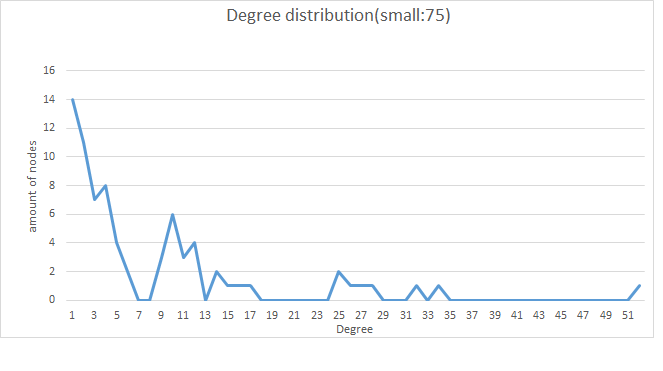
\includegraphics[width=\textwidth]{DDsmall}
		\caption{Degree distribution of small graph} 
		\label{fig:smallDegree}
	\end{subfigure}
	\begin{subfigure}{0.3\textwidth}
		\includegraphics[width=\textwidth]{DDmedium}
		\caption{Degree distribution of medium graph} 
		\label{fig:mediumDegree}
	\end{subfigure}
	\begin{subfigure}{0.3\textwidth}
		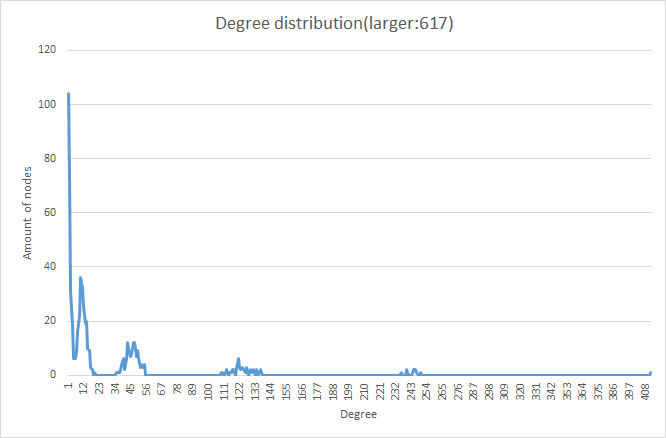
\includegraphics[width=\textwidth]{DDlarge}
		\caption{Degree distribution of large graph} 
		\label{fig:largeDegree}
	\end{subfigure}
	\caption{Degree distribution of the graph}
	\label{fig:DD}
\end{figure}



\section{The simulation}
We wish to see how each algorithm scales with the increase of the graph size and compare the result from each algorithm to each other. We implemented the four different algorithm and ran the simulation on three different sized network. The simulation would first choose a set of $k$ seed nodes as initial activated nodes. For each step, the activated nodes would propagate the activation to their neighbors. Each node can only try to activate their neighbor once. Since ICM have a global probability, to reduce the random effect of the propagation, for each new $k$, we would run the simulation 50 times with the same seed and find the average spread of that seed node. We created two different stop criteria for the simulation. The first simulation would stop only when there are no more nodes to activate, either since all the node that can be activated have been tested or somewhere in the network, the activation died out. The other criteria was after a specific amount of step, the simulation would stop.

For the second simulation, we choose to find the average "Step" the greedy algorithm would take before no more nodes can be activated and set the limit to 70\% of that value. For the small graph, we set the limit to 15 step, for the medium graph the limit was at 125, and the large graph was 190 step. We choose to have a global probability of 0.05 to activate the neighbors. The resulted graph can be seen in Figure \ref{fig:graph}.  


\begin{figure}[!ht]
	\begin{subfigure}{0.3\textwidth}
		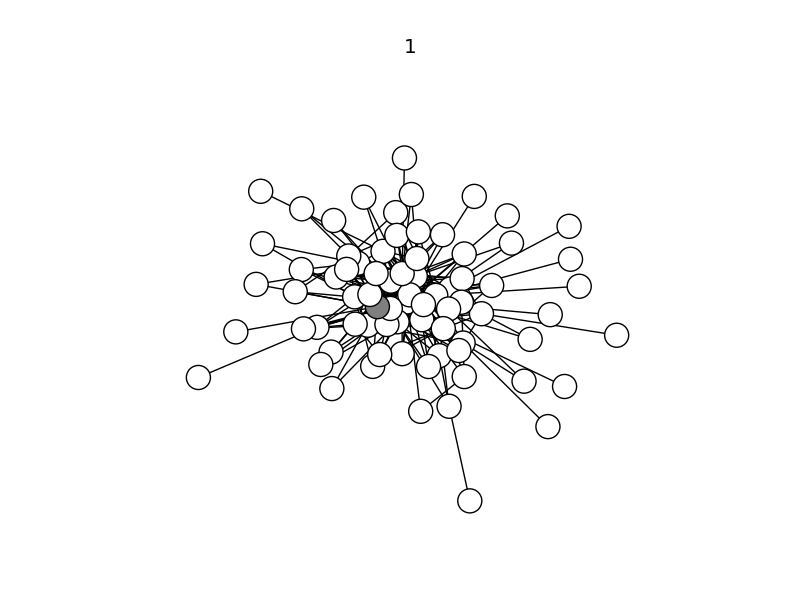
\includegraphics[width=\textwidth]{graph_small}
		\caption{The small graph} 
		\label{graphS}
	\end{subfigure}
	\begin{subfigure}{0.3\textwidth}
		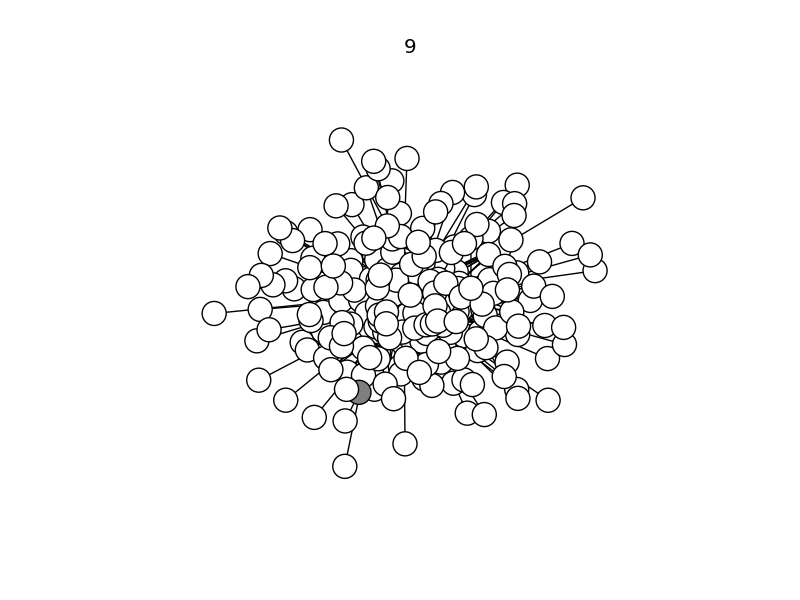
\includegraphics[width=\textwidth]{graph_medium}
		\caption{The medium graph} 
		\label{graphM}
	\end{subfigure}
	\begin{subfigure}{0.3\textwidth}
		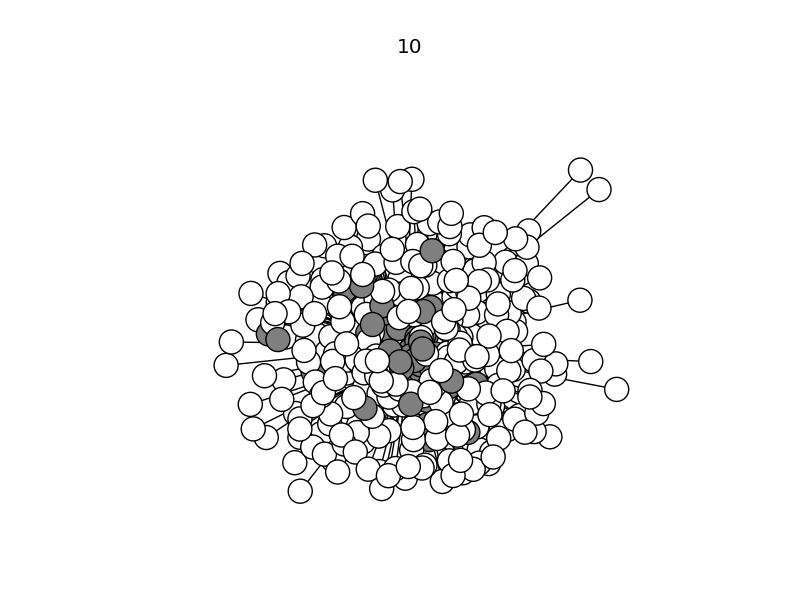
\includegraphics[width=\textwidth]{graph_large}
		\caption{The large graph} 
		\label{fig:graphL}
	\end{subfigure}

	\caption{The different graphs we ran our simulation through}
	\label{fig:graph}
\end{figure}

